\documentclass{article}

\usepackage[utf8]{inputenc}
\usepackage{natbib}
\usepackage{graphicx}
\usepackage{hyperref}
\usepackage{xcolor}
\usepackage[margin=1in]{geometry}

\title{
    Smart Dam \\
    \large Applicazioni e Servizi Web
}

\author{\href{mailto:emalama@studio.unibo.it}{Emanuele Lamagna} - 000725342\\\href{mailto:filippo.barbari@studio.unibo.it}{Filippo Barbari} - 000123456\\\href{mailto:filippo.benvenuti3@studio.unibo.it}{Filippo Benvenuti} - 0001027545}
\date{\today}

\begin{document}

\maketitle
\section*{Introduzione}\label{sec:intro}
L'idea è di rivisitare un progetto svolto nell'ambito del corso di Sistemi Embedded e Internet of Things, che consisteva nella simulazione di una diga smart e monitoraggio del livello idrometrico di un fiume. il sistema era composto da 5 sottosistemi, descritti dall'immagine \ref{fig:dam-scheme}.
\begin{figure}[h!]
	\centering
	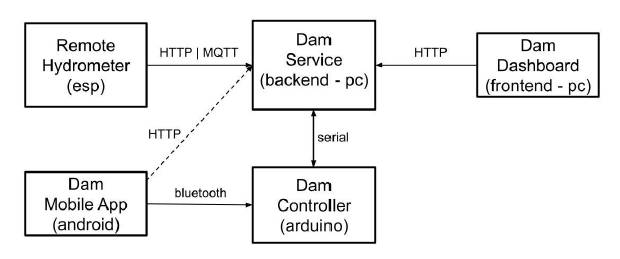
\includegraphics[scale=0.7]{dam-scheme.png}
	\caption{Diagramma dei componenti di DAM}
	\label{fig:dam-scheme}
\end{figure}
L'idea è di rifare da zero backend e frontend utilizzando Node e Vue, oltre all'utilizzo di MongoDB per il salvataggio dei dati. Inoltre per evitare di riesumare Arduino, ESP e l'applicazione mobile (che non concernono il progetto d'esame) simuleremo i sensori/attuatori abilitando tutti i componenti del team allo sviluppo e test del progetto.

\section{Requisiti}
\textcolor{red}{\textbf{Descrizione delle caratteristiche e funzionalità che il sistema prevede.}} % To remove!
Tenendo in considerazione le anticipazioni al capitolo \ref{sec:intro} il sistema si riduce a 3 principali componenti:
\begin{enumerate}
	\item \textbf{Dam Backend} (service):
	\begin{itemize}
		\item Salvataggio dati rilevati dai sensori.
		\item Esposizione interfaccia API accessibile tramite HTTP per lettura/salvataggio dati sensori.
	\end{itemize} 
	\item \textbf{Dam Frontend} (Dashboard):
	\begin{itemize}
		\item Grafico real-time relativo all'andamento del livello dell'acqua:
		\begin{itemize}
			\item Linea blu livello corrente acqua.
			\item Linea rossa d'allarme.
			\item Linea gialla d'allerta.
			\item Scelta periodo di aggiornamento grafico.
			\item Possibilità di forzare l'aggiornamento manualmente.
			\item Altri grafici mostranti dati su: temperatura dell'acqua, temperatura esterna, umidità, pressione atmosferica e pioggia.
		\end{itemize}
		\item Panoramic viewer della diga a 360°:
		\begin{itemize}
			\item Zoom in e out, possibilità di entrare in modalità full-scren.
			\item Visione colorata dei livelli di allerta sulla diga.
			\item Ultimo livello rilevato dell'acqua visualizzato sulla diga in tempo reale.
		\end{itemize}
		\item Homepage accessibile, con particolare riguardo a:
		\begin{itemize}
			\item Persona cieca.
			\item Persona ipovedente.
			\item Persona daltonica.
		\end{itemize}
	\end{itemize}
	\item \textbf{Dam Sensor} (Esp, arduino, mobile):
	\begin{itemize}
		\item Simulazione sensori e attuatori IOT:
		\begin{itemize}
			\item Sensore livello dell'acqua.
			\item Sensore del tempo atmosferico.
			\item Attuatore apertura diga.
		\end{itemize}
	\end{itemize}
\end{enumerate}

\section{Design}
\textcolor{red}{\textbf{Design dell'architettura del sistema e delle interfacce utente.}}

\begin{figure}[h!]
\centering
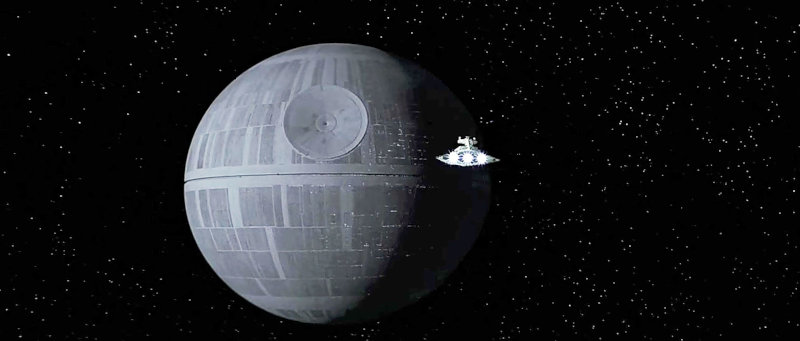
\includegraphics[scale=0.44]{deathStar2.jpg}
\caption{Death Star}
\label{fig:deathstar}
\end{figure}

\section{Tecnologie}
\textcolor{red}{\textbf{Tecnologie adottate e motivazioni.}}
\subsection{Node}
\subsection{Vue}
\subsection{ApexChart}
\subsection{Photo Sphere Viewer}
\subsection{Axios}
\subsection{MongoDB}
\subsection{Docker}

\section{Codice}
\textcolor{red}{\textbf{Solo aspetti rilevanti.}}
\textcolor{green}{\textbf{Qui potremmo metterci la parte di codice che tira su l'immagine a 360 e il graph component.}}

\section{Test}
\textcolor{red}{\textbf{Test effettuati sul codice e test con utenti.}}
\textcolor{green}{\textbf{I test di accessibilità sulla homepage, SBAM!\\Simuliamo di averlo fatto provare a Mosè al posto che separare le acque.}}

\section{Deployment}
\textcolor{red}{\textbf{Rilascio, installazione e messa in funzione.}}
\textcolor{green}{\textbf{Docker, docker e ancora docker, mini tutorial su come mettere tutto in esecuzione, gioia di vivere.}}

\section{Conclusioni}
\textcolor{red}{\textbf{Conclusioni}}
\textcolor{green}{Le relazioni d'esempio sono lunghe un botto mi viene da piangere.}

\bibliographystyle{plain}
\bibliography{references}
\end{document}
